\documentclass[12pt, a4paper]{article}
\title{Chapter 1}
\author{Maciej Harbuz}
\usepackage{amssymb}
\usepackage{amsmath}
\usepackage{tikz} 
\usepackage{import}
\usepackage{float}
\newcommand{\Mod}[1]{\ (\mathrm{mod}\ #1)}
\usetikzlibrary{automata, positioning, arrows}
\includeonly{chapter01-problems-160-169.tex}
\tikzset{
    ->, % makes the edges directed
    every state/.style={thick, fill=gray!15}, % sets the properties for each ’state’ node
    node distance=2.5cm, % specifies the minimum distance between two nodes. Change if necessary.
    initial text=$ $, % sets the text that appears on the start arrow
    >=stealth, % makes the arrow heads bold
}

\begin{document}

\maketitle

\section{Exercises}
\begin{enumerate}

    \item [1.19]
          Use the procedure described in Lemma 1.55 to convert the following regular expressions to nondeterministic finite automata.
          \begin{enumerate}
              \item $(0 \cup 1)^\ast000(0 \cup 1)^\ast$
              \item $(((00)^\ast(11)) \cup 01)^\ast$
              \item $\emptyset$
          \end{enumerate}

\end{enumerate}

\begin{enumerate}

    \item [1.22]
          In certain programming languages, comments appear between delimiters such as \slash\# and \#\slash .Let $C$ be the language of all valid delimited comment strings. A member of $C$ must begin with \slash \# and end with \# \slash but have no intervening \# \slash. For simplicity, assume that the alphabet for $C$ is $\Sigma=\{a,b,\text{/},\text{\#}\}$.
          \begin{enumerate}
              \item Give a DFA that recognizes $C$.
                    \begin{figure}[H]
                        \centering
                        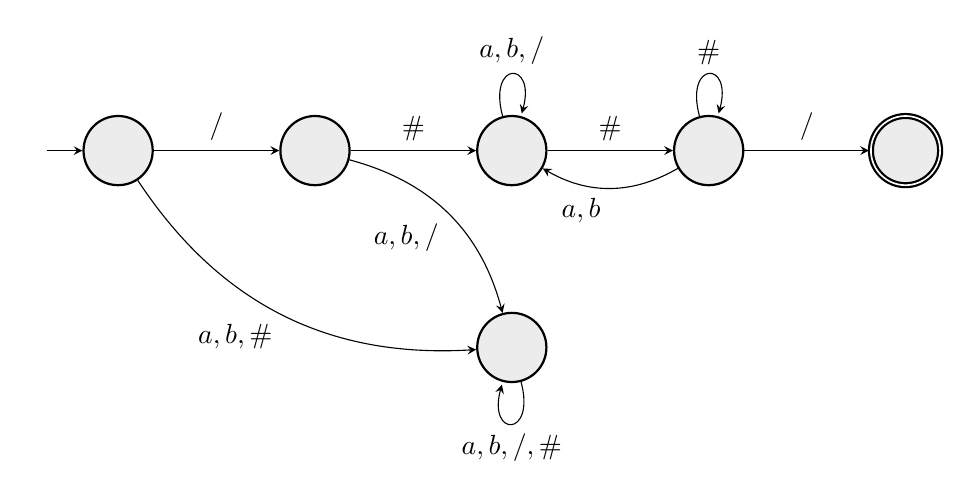
\begin{tikzpicture}[
                            ]
                            \node[state, initial] (q0) {};
                            \node[state, right of=q0] (q1) {};
                            \node[state, right of=q1] (q2) {};
                            \node[state, right of=q2] (q3) {};
                            \node[state, accepting, right of=q3] (q4) {};
                            \node[state, below of=q2] (q5) {};
                            \draw
                            (q0) edge[above] node{$\slash$} (q1)
                            (q1) edge[above] node{$\#$} (q2)
                            (q2) edge[loop above, above] node{$a,b,\slash$} (q2)
                            (q2) edge[above] node{$\#$} (q3)
                            (q3) edge[above] node{$\slash$} (q4)
                            (q0) edge[bend right, below left] node{$a,b,\#$} (q5)
                            (q1) edge[bend left, below left] node{$a,b,\slash$} (q5)
                            (q3) edge[bend left, below left] node{$a,b$} (q2)
                            (q3) edge[loop above, above] node{$\#$} (q3)
                            (q5) edge[loop below, below] node{$a,b,\slash,\#$} (q5);
                        \end{tikzpicture}
                        \caption{DFA recognizing $C$}
                    \end{figure}
              \item Give a regular expression that generates $C$.
                    $$\slash \#(a \cup b \cup \slash \cup (\#^\ast(a \cup b)))^\ast \# \slash $$
          \end{enumerate}
\end{enumerate}

\begin{enumerate}

    \item [1.31]
          For any string $w = w_1w_2\ldots w_n$, the reverse of $w$, written $w^\mathbb{R}$, is the string $w$ in reverse order, $w_n \ldots w_2w_1$. For any language A, let $A^\mathbb{R} = \{w^\mathbb{R}| w \in A\}$. Show that if $A$ is regular, so is $A^\mathbb{R}$.

          
\end{enumerate}

\begin{enumerate}

    \item [1.36]
          Let $B_n = \{a^k |  ~k~\text{is a multiple of} ~n\}$. Show that for each $n \ge 1$, the language $B_n$ is regular.

          Lets construct NFA accepting

          For $n = 2$:
          \begin{figure}[H]
              \centering
              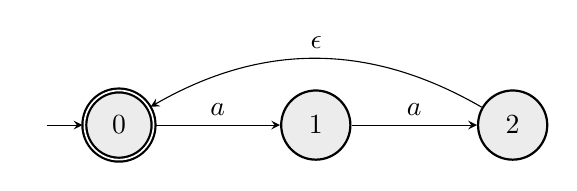
\begin{tikzpicture}[
                  ]
                  \node[state, initial, accepting] (q0) {$0$};
                  \node[state, right of=q0] (q1) {$1$};
                  \node[state, right of=q1] (q2) {$2$};
                  \draw
                  (q0) edge[above] node{$a$} (q1)
                  (q1) edge[above] node{$a$} (q2)
                  (q2) edge[bend right, above] node{$\epsilon$} (q0);
              \end{tikzpicture}
              \caption{NFA recognicing $B_2$}
          \end{figure}

          \begin{figure}[H]
              \centering
              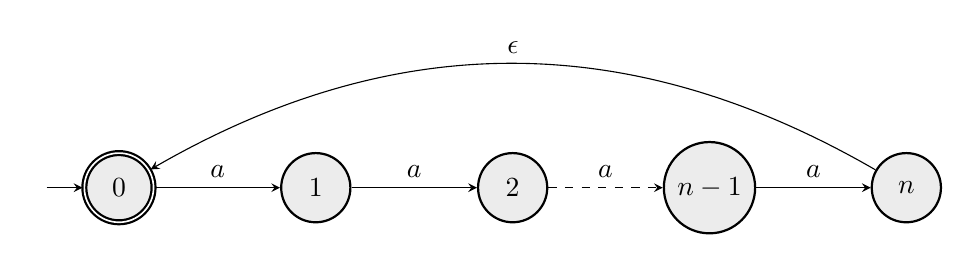
\begin{tikzpicture}[
                  ]
                  \node[state, initial, accepting] (q0) {$0$};
                  \node[state, right of=q0] (q1) {$1$};
                  \node[state, right of=q1] (q2) {$2$};
                  \node[state, right of=q2] (qe1) {$n-1$};
                  \node[state, right of=qe1] (qe) {$n$};
                  \draw
                  (q0) edge[above] node{$a$} (q1)
                  (q1) edge[above] node{$a$} (q2)
                  (q2) edge[above, dashed] node{$a$} (qe1)
                  (qe1) edge[above] node{$a$} (qe)
                  (qe) edge[bend right, above] node{$\epsilon$} (q0);
              \end{tikzpicture}
              \caption{NFA recognicing $B_n$}
          \end{figure}

    \item [1.37]
          Let $C_n = \{x~ |~ x~ \text{is a binary number that is a multiple of} ~n\}$. Show that for each $n \ge 1$, the language $C_n$ is regular.

          Lets build $DFA_C$ recognizing $C_n$:

          $DFA_C = (Q, \Sigma, \delta, q_0, F)$
          \begin{itemize}
              \item $Q = \{0', 1', 2', \ldots, (n-1)'\}$
              \item $\Sigma = \{0, 1\}$
              \item $q_0 = 0'$
              \item $F = \{0'\}$
              \item $\delta$ is defined as follows:
                    \begin{align*}
                        \delta(q', 0) & = 2q \Mod{n}                                   \\
                        \delta(q', 1) & = (2q + 1) \Mod{n} = (2q \Mod{n} + 1 ) \Mod{n}
                    \end{align*}
                    where q is the integer part of $q'$.
          \end{itemize}
          We build DFA recognizing $C_n$ so $C_n$ is regular.

          Idea

          $i\text{-th}$ state represents integers which modulo from dividing by $n$ is $i$, because $n$ is multiple of $n$.

          \begin{figure}[H]
              \centering
              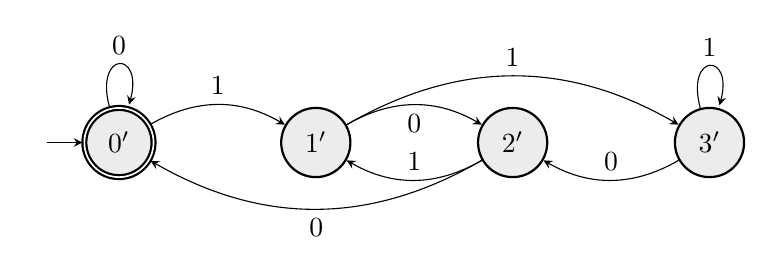
\begin{tikzpicture}[
                  ]
                  \node[state, initial, accepting] (q0) {$0'$};
                  \node[state, right of=q0] (q1) {$1'$};
                  \node[state, right of=q1] (q2) {$2'$};
                  \node[state, right of=q2] (q3) {$3'$};
                  \draw
                  (q0) edge[loop above] node{$0$} (q0)
                  (q0) edge[bend left, above] node{$1$} (q1)
                  (q1) edge[bend left, below] node{$0$} (q2)
                  (q1) edge[bend left, above] node{$1$} (q3)
                  (q2) edge[bend left, below] node{$0$} (q0)
                  (q2) edge[bend left, above] node{$1$} (q1)
                  (q3) edge[bend left, above] node{$0$} (q2)
                  (q3) edge[loop above] node{$1$} (q3);
              \end{tikzpicture}
              \caption{$DFA_C$ for $n = 4$}
          \end{figure}

          \begin{table}[H]
              \centering
              \begin{tabular}{|r|r|r|r|}
                  \hline
                  $0'$: mod 4 = 0 & $1'$: mod  4 = 1 & $2'$: mod 4 = 2 & $3'$: mod 4 = 3 \\
                  \hline
                  $0 = (0)_2$     & $1 = (1)_2$      & $2 = (10)_2$    & $3 = (11)_2$    \\
                  $4 = (100)_2$   & $5 = (101)_2$    & $6 = (110)_2$   & $7 = (111)_2$   \\
                  $8 = (1000)_2$  & $9 = (1001)_2$   & $10 = (1010)_2$ & $11 = (1011)_2$ \\
                  \ldots          & \ldots           & \ldots          & \ldots          \\
                  \hline
              \end{tabular}
          \end{table}

    \item [1.38]

          An all-NFA $M$ is a 5-tuple $(Q,\Sigma,\delta,q_0,F)$ that accepts $x \in \Sigma^\ast$ if every possible state that $M$ could be in after reading input $x$ is a state from $F$. Note, in contrast, that an ordinary NFA accepts a string if some state among these possible states is an accept state. Prove that all-NFAs recognize the class of regular languages.

          In procedure to change NFA to DFA just change step which marks state as accepting when state of DFA corresponds to states of NFA with at least one is acccepting to accepting only when all states are accepting.

          Now we have DFA avvepting the same language as all-NFA $M$ so language is regular.
    \item [1.39]
          The construction in Theorem 1.54 shows that every GNFA is equivalent to a GNFA with only two states. We can show that an opposite phenomenon occurs for DFAs. Prove that for every $k > 1$, a language $A_k \subseteq \{0,1\}^\ast$ exists that is recognized by a DFA with $k$ states but not by one with only $k-1$ states.
    \item [1.40]
          Recall that string $x$ is a \textbf{prefix} of string $y$ if a string $z$ exists where $xz = y$, and that $x$ is a \textbf{proper prefix} of $y$ if in addition $x \neq y$. In each of the following parts, we define an operation on a language $A$. Show that the class of regular languages is closed under that operation.
          \begin{itemize}
              \item $L = \text{NOPREFIX}(A)=\{w \in A~|~\text{no proper prefix of } w~ \text{is a member of}~ A\}$.

                    Let be DFA $M = (Q, \Sigma, \delta, q_0, F)$ recognizes A (as A is regular language).

                    We need to construct $L$ which contains strings so that DFA $M$ will go to accepting state only at the end of processing string. In other words for all $w = w_1w_2\ldots w_n \in A$, $\delta(q_{i-1}, w_i) = q_{i}$ and $q_i \in F$ only for $i = n$.

                    Let $\overline{L} = \overline{NOPREFIX(A)}$

                    $\overline{L} = \{w \in A~|~\text{there is a proper prefix of } w~ \text{is a member of}~ A\}$.

                    $\overline{L} = \{w \in A~|~\text{there is}~ x \in A~\text{ and }~ z \in \Sigma^\ast  | w = xz\}$.

              \item $\text{NOEXTEND}(A)=\{w \in A~|~w~ \text{is not the proper prefix of any string in}~ A\}$.
          \end{itemize}
\end{enumerate}

\begin{enumerate}

    \item [1.41]

          For languages $A$ and $B$,let the \textbf{perfect shuffle} of $A$ and $B$ be the language $\{w~|~ w = a_1b_1\ldots a_kb_k , \text{where} a_1\ldots a_k \in A \text{and} b_1 \ldots b_k \in B, each a_i,b_i \in \Sigma\}$. Show that the class of regular languages is closed under perfect shuffle.

          TODO - double check this solution

          Let $A$ and $B$ be regular languages. Then there exist DFAs $M_A$ and $M_B$ that accept $A$ and $B$, respectively. We construct a DFA $M$ that accepts the perfect shuffle of $A$ and $B$.

          Let $M_A = (Q_A,\Sigma,\delta_A,q_{0A},F_A)$ and $M_B = (Q_B,\Sigma,\delta_B,q_{0B},F_B)$. Let $Q = Q_A \times Q_B$, $q_0 = (q_{0A},q_{0B})$, and $F = F_A \times F_B$. The transition function $\delta$ is defined as follows: for each $q \in Q$ and $a \in \Sigma$, $\delta(q,a) = (\delta_A(q_A,a),\delta_B(q_B,a))$.

          We claim that $L(M) = A \circ B$. Let $w = a_1b_1\ldots a_kb_k \in A \circ B$. Then there exists a sequence of states $r_0,r_1,\ldots,r_k$ such that $r_0 = q_0$, $r_k \in F$, and $\delta(r_{i-1},a_i) = r_i$ for $i = 1,\ldots,k$. Let $r_i = (r_{iA},r_{iB})$. Then $r_{iA} \in Q_A$ and $r_{iB} \in Q_B$. Since $r_k \in F$, $r_{kA} \in F_A$ and $r_{kB} \in F_B$. Thus $a_1\ldots a_k \in A$ and $b_1\ldots b_k \in B$. Therefore $w \in A \circ B$.

          Conversely, let $w = a_1\ldots a_kb_1\ldots b_k \in A \circ B$. Then $a_1\ldots a_k \in A$ and $b_1\ldots b_k \in B$. Let $r_i = (r_{iA},r_{iB})$ for $i = 0,\ldots,k$. Then $r_0 = q_0$, $r_k \in F$, and $\delta(r_{i-1},a_i) = r_i$ for $i = 1,\ldots,k$. Therefore $w \in L(M)$.


    \item [1.42]
    \item [1.43]
    \item [1.44]
    \item [1.45]
    \item [1.46]
    \item [1.47]
    \item [1.48]
    \item [1.49]

\end{enumerate}

\begin{enumerate}

      \item [1.50]
      \item [1.51]
      \item [1.52]
      \item [1.53]
      \item [1.54]
      \item [1.55]
      \item [1.56]
      \item [1.57]
      \item [1.58]
      \item [1.59]

\end{enumerate}

\begin{enumerate}

      \item [1.60]
            
            
            Let $\Sigma =\{a,b\}$. For each $k \ge 1$, let $C_k$ be the language consisting of all strings that contain an a exactly $k$ places from the right-hand end. Thus $C_k = \Sigma^\ast a \Sigma^{k-1}$. Describe an NFA with $k+1$ states that recognizes $C_k$ in terms of both a state diagram and a formal description.
            
      \item [1.61]
            
            Consider the languages $C_k$ defined in Problem 1.60. Prove that for each $k$, no DFA can recognize $C_k$ with fewer than $2k$ states.
            
      \item [1.62]
            
            Let $\Sigma =\{a,b\}$. For each $k \ge 1$, let $D_k$ be the language consisting of all strings that have at least one $a$ among the last $k$ symbols. Thus $D_k = \Sigma^\ast a(\Sigma \cup \epsilon)^{k-1}$. Describe a DFA with at most $k+1$ states that recognizes $D_k$ in terms of both a state diagram and a formal description.
            
      \item [1.63]
            
            \begin{enumerate}
                  \item Let $A$ be an infinite regular language. Prove that $A$ can be split into two infinite disjoint regular subsets.
                  \item Let $B$ and $D$ be two languages. Write $B \Subset D$ if $B \subseteq D$ and $D$ contains infinitely many strings that are not in $B$. Show that if $B$ and $D$ are two regular languages where $B \Subset D$, then we can find a regular language $C$ where $B \Subset C \Subset D$.
            \end{enumerate}
            
      \item [1.64]
            
            Let $N$ be an NFA with $k$ states that recognizes some language $A$.
            \begin{enumerate}
                  \item Show that if $A$ is non empty, $A$ contains some string of length at most $k$.
                  \item Show, by giving an example, that part (a) is not necessarily true if you replace both $A$’s by $\overline{A}$.
                  \item Show that if $\overline{A}$ is non empty, $\overline{A}$ contains some string of length at most $2k$.
                  \item Show that the bound given in part (c) is nearly tight; that is, for each $k$, demonstrate an NFA recognizing a language $\overline{A_k}$ where $\overline{A_k}$ is non empty and where $\overline{A_k}$’s shortest member strings are of length exponential in $k$. Come as close to the bound in (c) as you can.
            \end{enumerate}
            
      \item [1.65]
            
            Prove that for each $n > 0$, a language $B_n$ exists where
            \begin{enumerate}
                  \item $B_n$ is recognizable by an NFA that has $n$ states, and
                  \item if $B_n = A_1 \cup \ldots \cup A_k$, for regular languages $A_i$, then at least one of the $A_i$ requires a DFA with exponentially many states.
            \end{enumerate}
            
      \item [1.66]
            
            A \textbf{homomorphism} is a function $f: \Sigma \longrightarrow \Gamma^\ast$ from one alphabet to strings over another alphabet. We can extend $f$ to operate on strings by defining $f(w)= f(w_1)f(w_2) \ldots f(w_n)$, where $w = w_1 w_2 \ldots w_n$ and each $w_i \in \Sigma$. We further extend $f$ to operate on languages by defining $f(A)=\{f(w)|~ w \in A\}$, for any language $A$.
            
            \begin{enumerate}
                  \item Show, by giving a formal construction, that the class of regular languages is closed under homomorphism. In other words, given a DFA $M$ that recognizes $B$ and a homomorphism $f$, construct a finite automaton $M'$ that recognizes $f(B)$. Consider the machine $M'$ that you constructed. Is it a DFA in every case?
                  \item Show, by giving an example, that the class of non-regular languages is not closed under homomorphism.
            \end{enumerate}
            
      \item [1.67]
            
            Let the rotational closure of language $A$ be $RC(A)=\{yx|~ xy \in A\}$.
            \begin{enumerate}
                  \item Show that for any language $A$, we have $RC(A)=RC(RC(A))$.
                  \item Show that the class of regular languages is closed under rotational closure.
            \end{enumerate}
            
            Every string $s$ in language $RC(A)$ has a form $yx$ where $xy$ is in language $A$. 
            If $\epsilon \in A$ then $A \subseteq RC(A)$. So $RC(A) \subseteq RC(RC(A))$.

            Suppose $w \in RC(RC(A))$ and $w = yx$ where $xy \in RC(A)$. Then $xy = zt$ where $zt \in A$. So $yx = zt$ and $zt \in A$. Therefore $w \in RC(A)$.

            
      \item [1.68]
            
            In the traditional method for cutting a deck of playing cards, the deck is arbitrarily split two parts, which are exchanged before reassembling the deck. In a more complex cut, called Scarne’s cut, the deck is broken into three parts and the middle part in placed first in the reassembly. We’ll take Scarne’s cut as the inspiration for an operation on languages.
            For a language $A$, let $CUT(A)={yxz|~xyz \in A}$.
            \begin{enumerate}
                  \item Exhibit a language $B$ for which $CUT(B)= CUT(CUT(B))$.
                  \item Show that the class of regular languages is closed under $CUT$.
            \end{enumerate}
            
            
      \item [1.69]
            
            Let $Sigma=\{0,1\}$. Let $WW_k = \{ww|~ w \in \Sigma^\ast~ \text{and}~ w~ \text{is of length}~ k\}$.
            \begin{enumerate}
                  \item Showthat foreach $k$, no DFA can recognize $WW_k$ with fewer than $2^k$ states.
                  \item Describe a much smaller NFA for $\overline{WW_k}$, the complement of $WW_k$.
            \end{enumerate}
            
\end{enumerate}



\end{document}
